\section{XML}

\begin{figure}[h]
    \centering
    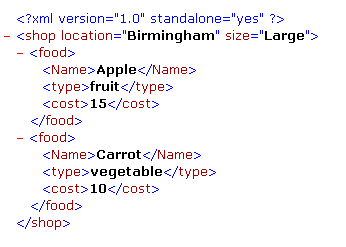
\includegraphics[width=0.6\textwidth]{imagens/ExampleXML.png}
    \caption{Exemplo de arquivo XML. \\Fonte: https://www.jonathanmedd.net/2009/12/powershell-2-0-one-cmdlet-at-a-time-21-select-xml.html}
    \label{fig:xml_example}
\end{figure}

\subsection{O que é?}

O XML (Extensible Markup Language) é uma linguagem de marcação responsável por descrever classes de dados para ampla distribuição na internet, focada em ser legível tanto por humanos quanto por maquinas, e em permitir a interoperabilidade entre diferentes sistemas e aplicações\cite{bray2000xml}.

Uma das características centrais do XML é que suas tags (marcadores semânticos) nao são pré-definidos, isso significa que fica aberto para o usuário de XML descrever sua estrutura de dados da melhor forma que lhe convenha \cite{mozillaxml}. A união dessa liberdade semântica com a padronização da sintaxe inerente ao XML o torna uma ferramenta eficaz em distribuir dados na internet.

Existem 3 possíveis estados para um documento XML\cite{ibmxml}:
\begin{itemize}
  \item Inválido: Não segue as regras de sintaxe de XML. Caso um documento XML nao siga as regras semânticas definidas no DTD (Document Type Definition) ou no schema definido pelo desenvolvedor isso também torna inválido.
  \item Well formed: Segue as regras de sintaxe do XML, mas não possui regras semanticas definidas num DTD ou schema.
  \item Válido: Segue regras sintáticas e semânticas.
\end{itemize}

\subsection{Well-formedness - A Sintaxe do XML}

Uma das características marcantes do XML em relação a outras linguagens de marcação (HTML, usado para mostrar conteúdo em paginas web, e seu ancestral direto, o SGML), é a de que a leitura de um documento XML deve ser não ambígua, isso garante que não ocorrerão erros durante a leitura do XML, para isso, definem-se uma coleção de regras que tem como objetivo garantir essa facilidade de leitura do documento XML \cite{computerphile}.

\bigskip

Alguns exemplos dessas regras são:
\begin{itemize}
  \item Posicionamento da declaração de XML: um header inicial que define metadados para a leitura do arquivo, é opcional, mas caso esteja presente, precisa estar na primeira linha do arquivo.
  \item Presença de um elemento raiz: o elemento raiz deve encapsular todos os outros elementos.
  \item Elementos não podem se intercalar: um elemento contem outro completamente, tanto sua abertura quanto fechamento.
  \item XML é case sensitive: não é possível fechar uma tag minuscula em maiúsculo.
\end{itemize}

\newline
\smallskip

Demonstração:

% TODO: ver esta grande merda
    % eu queria um tema haxxor
\begin{minted}[
    % style=monokai,
    % bgcolor=monokai,
    linenos
]{xml}
<!-- Esta é a sintaxe de comentários em xml -->

<!-- Declaração de XML -->
<?xml version="1.0" encoding="ISO-8859-1" standalone="no"?>

<!-- Exemplo de quebra do elemento raiz -->
<section_1>
  Hello, World!
</section_1>
<section_2>
  <!-- Exemplo de elementos intercalando-se indevidamente -->
  <p>
    <b>I 
    <i>really love
    </b> XML.
    </i>
  </p>
  
  <!-- Exemplo de tag quebrando a regra de case sensitive -->
  <h1>Elements are case sensitive</H1>
</section_2>
\end{minted}


\subsection{DTD e Schema - A Semântica do XML}

DTD (Document Type Definition) consiste de uma gramática que estrutura de que forma as tags se relacionam entre si. Mencionamos anteriormente que uma das forças do XML é a liberdade do usuário em customizar o documento para seu caso de uso, entretanto, em meio a um mesmo caso de uso, é útil possuir constrições para garantir que diferentes fontes para um mesmo escopo estejam padronizadas: quais atributos podem ser aplicados a cada elemento, em que ordem podem aparecer, quais relações hierárquicas são permitidas\cite{wikixml}.

Exemplo de um DTD Interno (linhas 2 até 7):
\begin{minted}[
    % style=monokai,
    % bgcolor=monokai,
    linenos
]{xml}
 <?xml version="1.0"?>
<!DOCTYPE note [
<!ELEMENT note (to,from,heading,body)>
<!ELEMENT to (#PCDATA)>
<!ELEMENT from (#PCDATA)>
<!ELEMENT heading (#PCDATA)>
<!ELEMENT body (#PCDATA)>
]>
<note>
<to>Tove</to>
<from>Jani</from>
<heading>Reminder</heading>
<body>Don't forget me this weekend</body>
</note> 
\end{minted}

Basicamente, definimos o doctype note, e o elemento note, que pode conter as tags (to,from,heading,body) internamente, e estas, todas usam o tipo primitivo #PCDATA (significando \textit{parsed character data})

Acima, fomos apresentados ao DTD Interno, que possui esse nome por ser definido dentro do próprio XML que o usa, uma outra forma de definir o DTD seria apontar para um arquivo encontrado localmente\cite{wikidtd}:

\begin{minted}[
    % style=monokai,
    % bgcolor=monokai,
    linenos
]{xml}
<!DOCTYPE note SYSTEM note.dtd>
\end{minted}

Dentro de note.dtd possuiríamos os mesmos elementos que usamos no exemplo acima por exemplo. Também é possível usar DTD's instanciadas publicamente, muito como faríamos com a importação de bibliotecas em uma linguagem de programação\cite{publicdtd}:

\begin{minted}[
    % style=monokai,
    % bgcolor=monokai,
    linenos
]{xml}
<!DOCTYPE html PUBLIC "-//W3C//DTD XHTML 1.0 Transitional//EN">
\end{minted}

Uma alternativa ao DTD é o Schema, que vai possuir a mesma contextualização, porém, será muito mais poderoso devido a algumas propriedades adicionais que possui sobre o DTD\cite{wikixmlschema}:

\begin{itemize}
  \item Uso de namespaces.
  \item Maior flexibilidade na definição de restrições com o uso de regex, ranges numéricos e enumeradores.
  \item Mais possibilidades para definição de campos unicos, ao contrário de ID e IDREF em DTDS, podem ser definidos em qualquer parte do documento, serem de qualquer tipo de dado, e podem se referir tanto a elementos quanto a conteúdo.
\end{itemize}

Outro fator interessante é que o schema é construido sobre uma sintaxe em XML! Tornando o uso mais legível e intuitivo:

\begin{minted}[
    % style=monokai,
    % bgcolor=monokai,
    linenos
]{xml}
<xs:element name="note">

<xs:complexType>
  <xs:sequence>
    <xs:element name="to" type="xs:string"/>
    <xs:element name="from" type="xs:string"/>
    <xs:element name="heading" type="xs:string"/>
    <xs:element name="body" type="xs:string"/>
  </xs:sequence>
</xs:complexType>

</xs:element> 
\end{minted}

% implicações do xml
\subsection{Quais as Implicações?}

O XML é um padrão de definição de dados amplamente utilizado ao longo da internet, isso fez com que fosse possível que desenvolvedores pudessem transmitir informações críticas por meio de API's, ampliando a comunicação de serviços e permitindo a construção conjunta de soluções mais e mais complexas. Essa ampla utilização do XML fez com que diversas tecnologias fossem construídas em cima do XML, ja utilizando dos padrões definidos, tais como XHTML, MathML, SVG, XUL, XBL, RSS, e RDF\cite{mozillaxml}.

Também um agrupamento de especificações formou-se em torno do XML para ampliar e especificar os usos de XML\cite{wikixml}:

\begin{itemize}
  \item XPath (XML Path Language), uma linguagem para referenciação de componentes de um arquivo XML. O XPath é usado amplamente por outras especificação em XML e em bibliotecas de programação para busca de dados definidos em XML.
  \item XQuery (XML Query) é uma linguagem de consulta construida em cima de XPath e XML Schema que providencia métodos para acessar, manipular e retornar XML, o que a torna perfeita para uso em conjunto com bancos de dados em XML.
  \item XML Encryption que define uma sintaxe para criptografia de conteúdo em XML.
\end{itemize}

Concluindo, o advento do XML permitiu que a troca de dados pudesse ser simplificada, uma vez que foi possível que linguagens e programadores pudessem focar na construção do ecossistema ao construir ferramentas que pudessem interpretar e construir XML que pudesse ser amplamente distribuído. XML permite a construção de código e buscas eficientes, a presença de metadados contextualizantes em torno dos elementos de dados faz com que o programador encontre o que busca\cite{ibmxml}.
